\section{Linux系统编程}

\subsection{IO函数}
Linux系统当中,通常需要处理IO,而IO的处理,在Linux的函数当中,主要有4个函数:
\begin{itemize}
  \item open //fcntl.h
  \item write //unistd.h
  \item read //unistd.h
  \item close //unistd.h
\end{itemize}

实现简单的touch命令的功能
\begin{code-block}{c}
#include <stdio.h>
#include <unistd.h>
#include <fcntl.h>

int main(int argc, char * argv[])
{
        // 第3个参数可以直接写为0644
        int fd = open(argv[1], O_CREAT|O_WRONLY,
                S_IRUSR|S_IWUSR|S_IRGRP|S_IROTH);
        if (0>fd)
        {
                printf("Cannot create file %s\n", argv[1]);
                return -1;
        }
        printf("Create file %s success\n", argv[1]);
        close(fd);
        return 0;
}
\end{code-block}

但是,由于Linux操作系统本身存在umask(默认为022),因此,如果上述的第3个参数写作0777,
生成的文件的权限与umask进行亦或计算之后,实际上,文件的权限还是755,并不是我们所期待的
777。如果需要保持设置的权限与生成的文件权限完全一致,需要执行如下命令:
\begin{code-block}{bash}
umask 000
# 后续再执行代码,生成文件
\end{code-block}

Open函数只能生成普通文件,如果是管道、字符设备之类的,则无法使用open函数进行创建。
另外,如果只是需要打开文件,并不是创建文件,则open函数的第3个参数不需要。
除此之外,还需要注意一下,文件的打开模式
\begin{itemize}
  \item O\_TRUNC:覆盖文件
  \item O\_EXCL : 与O\_CREAT合用,如果对应文件已经存在,则提示错误
\end{itemize}

Open函数一旦调用,Linux内核会在内核空间打开3个文件描述符,分别是0,1,2。

而对应的,也可以利用write函数向打开的文件句柄当中写入内容
\begin{code-block}{c}
#include <stdio.h>
#include <unistd.h>
#include <fcntl.h>

int main(int argc, char * argv[])
{
        // 第3个参数可以直接写为0644
        int fd = open(argv[1], O_CREAT|O_RDWR,
                S_IRUSR|S_IWUSR|S_IRGRP|S_IROTH);
        if (0>fd)
        {
                printf("Cannot create file %s\n", argv[1]);
                return -1;
        }
        printf("Create file %s success\n", argv[1]);

        char msg[] = "hello world";
        write(fd, msg, sizeof(msg)/sizeof(char)); //会写入一个文件结束符,特殊符号
                                                  // 如果不需要,则将长度-1即可
        close(fd);
        return 0;
}
\end{code-block}

相应的,也可以利用read函数读取打开文件的内容:
\begin{code-block}{c}
#include <stdio.h>
#include <unistd.h>
#include <fcntl.h>
#include <string.h>

int main(int argc, char * argv[])
{
        int fd = open(argv[1], O_RDONLY);
        if (0>fd)
        {
                printf("Cannot open file %s\n", argv[1]);
                return -1;
        }
        printf("Open file %s success\n", argv[1]);

        size_t read_ret = 0;
#if 0
        // 连续多次读取,并非一次性读完
        size_t total = 0;
        char readbuf[128];
        while ((read_ret=read(fd, readbuf, 127))>0) // 每次只能读取max-1,否则末尾存在特殊字符,可能出现溢出
        {
                total += read_ret;
                printf("Read %d chars \n", read_ret);
                printf("The content of file is %s \n", readbuf);
                memset(readbuf, 0, 128);
        }
        printf("The total sizeof file is %d\n", total);
#else
        // 一次性读取
        char readbuf[1024];
        read_ret=read(fd, readbuf, 1024);
        printf("Read %d chars \n", read_ret);
        printf("The content of file is %s \n", readbuf);
#endif
        close(fd);
        return 0;
}
\end{code-block}

高级一点的,我们就可以使用read和write函数来实现一个简单的文件拷贝功能。
\begin{code-block}{c}
#include <stdio.h>
#include <unistd.h>
#include <fcntl.h>
#include <string.h>

int main(int argc, char * argv[])
{
        int readrd = 0, writefd = 0;
        if (0 >= (readrd = open(argv[1], O_RDONLY)))
        {
                printf("Cannot open the source file %s\n", argv[1]);
                return -1;
        }
        if (0 >= (writefd = open(
                argv[2], O_CREAT|O_TRUNC|O_WRONLY, 0644)))
        {
                printf("Cannot create the target file %s\n", argv[2]);
                return -1;
        }

        unsigned char buffer[128];
        memset(buffer, 0, 128);

        size_t readret = 0, writeret = 0;
        while(0 < (readret = read(readrd, buffer, 127)))
        {
                if (0 > (writeret = write(writefd, buffer, readret)))
                {
                        printf("Cannot write content to write file\n");
                        return -1;
                }
                memset(buffer, 0, 128);
        }

        close(readrd);
        close(writefd);
        return 0;
}
\end{code-block}

由于读取使用的是unsigned char,因此,上述文件也可以直接拷贝二进制文件。

\subsection{标准IO函数}
Linux的IO操作包括文件IO和标准IO。所谓的文件IO,即直接调用内核提供的系统调用函数,一般需要使用头文件unistd.h当中的函数;而
标准IO,则是通过调用C的库函数,间接的调用系统调用函数,通常的,使用的头文件stdio.h当中的函数。从功能上看,标准IO与文件IO是
相同的,但是,细节上,他们存在区别。
\begin{code-block}{c}
#include <stdio.h>
#include <unistd.h>

int main(int argc, char * argv[])
{
        char  buffer[] = "hello world";
        printf("stdio %s", buffer);
        write(1, buffer, 11);
        while(1);
        return 0;
}
\end{code-block}

上述代码编译之后,运行,只有hello world能够输出,而printf的stdio hello world则无法输出。问题在于缓存。
Linux程序当中存在几种缓存:
\begin{itemize}
  \item 用户空间缓存:即想从内核读写的数据,即上述代码当中buffer
  \item 内核空间缓存:没打开一个文件,内核会在内核空间开辟一块缓存,这个称之为内核空间的缓存
  \item 库缓存:标准IO的库函数的缓存
\end{itemize}

文件IO中的写,即是将用户空间的缓存写入到内核空间缓存当中;反之,文件IO的读,则是将内核空间的缓存读写到用户空间的缓存当中。
而调用标准IO之后,数据会从用户空间写入到库缓存,当写入的数据包含\textbackslash n时,或者库缓存空间写满时,才会向内核缓存空间提交数据。
因此,如果上述代码修改为
\begin{code-block}{c}
printf("stdio %s\n", buffer); //或者直接将库缓存写满
while(1);
\end{code-block}
则会直接输出。另外,库缓存的大小默认为1024个字节。

常用fgets,gets,printf,sprintf,fprintf,fputs,puts,scanf这些函数在遇到\textbackslash n或者写满缓存时,即
调用系统调用函数,称之为行缓存函数;而fread,fwrite只有在写满缓存之后再调用系统调用函数,这些则称之为全缓存函数;
而只要调用,则会将内容和数据写入到内核当中的函数,称之为无缓存函数,注意,stderr是无缓存的,而stdout则是行缓存的。
fclose函数在关闭文件之前,会刷新缓存当中的数据到文件当中。

需要注意的是fputc是缓存函数,但是,他不是行缓存函数,立即生效的话,需要使用fflush函数进行强制刷新。

除此之外,在标准IO当中,读取文件有可能会出现错误,而fgets函数读取正常时,返回读取到的内容,这个内容与fgets函数的第一个参数的结果一致,
如果读取错误,则会返回一个空指针(char)。但是无法准确判断这个错误是什么类型。判断错误的准确类型,可以使用feof和ferror函数进行判断。
前者表示读取到了文件末尾,而后一个则表示真的文件读取错误,如下代码所示:
\begin{code-block}{c}
FILE *fp = fopen("test.c")
char buffer[128];
char * read_ret = NULL;
read_ret = fgets(buffer, 128, fp);
if (NULL == read_ret)
{
        if(feof(fp))
        {
                printf("Read the end of file\n");
        }
        if(ferror(fp))
        {
                printf("Read error from the stream\n");
        }
}
\end{code-block}

与文件IO相对应的,标准IO使用fopen函数进行文件的创建和读写。但是需要特别注意的是,实际上,fopen函数创建的函数的权限始终是
666,但是由于umask的存在,因此,fopen函数创建的文件的最终权限为644。

全缓存函数fread和fwrite在使用的时候会调用syscall,写入到内核缓存当中,最后写入到硬件当中(文件)。同样的,我们也可以用fread和fwrite实现
Linux的cat命令,简单的如下:
\begin{code-block}{c}
if(NULL == (fp = fopen(argv[1], "rb")))
{
        printf("Cannot open the file %s\n", argv[1]);
        return -1;
}

unsigned char buffer[128];
memset(buffer, 0, 128);
while(0 < fread(buffer, sizeof(char), 128, fp))
{
        fwrite(buffer, sizeof(char), 128, stdout);
        memset(buffer, 0, 128);
        if(feof(fp))
        {
                printf("Read the the of file\n");
                break;
        }
}

fclose(fp); // 调用fflush,直接写入到内核缓存当中
return 0;
\end{code-block}

从执行效率上说,fgetc/fputc<fgets/fputs<fread/fwrite,主要原因在于fread基本都是在内核空间操作,效率有保证。因此,在有高效率要求的情况下,尽可能的使用fread和fwrite
作为IO的操作函数。

\subsection{目录IO}
除了文件IO和标准IO之外,Linux还提供了针对路径(目录)的IO操作函数,具体如图\nameref{fig:dirio}所示
\begin{figure}[H]
  \centering
  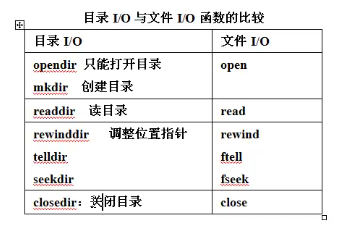
\includegraphics[scale=1]{dirio.png}
  \caption{Linux的目录IO函数}
  \label{fig:dirio}
\end{figure}

只是需要注意的是,mkdir函数在sys/stat.h当中,其他的函数大部分在dirent.h当中。目录的创建,可以使用如下的代码:
\begin{code-block}{c}
int ret = mkdir("zhangjl", 0777);
if(0 > ret)
{
        printf("Failed to create dir\n");
        return -1;
}
return 0;
\end{code-block}

而打开目录,则可以如下操作:
\begin{code-block}{c}
#include <dirent.h>

int main(int argc, char * argv[])
{
        DIR *dp = opendir("/root");
        if(NULL ==  dp)
        {
                printf("Failed to open dir\n");
                return -1;
        }

        closedir(dp);
        return 0;
}
\end{code-block}

读取目录内容,则可以使用readdir函数。由于readdir函数在多个头文件当中都有定义,此处应当使用dirent.h当中的函数。
具体的使用如下代码:
\begin{code-block}{c}
#include <stdio.h>
#include <dirent.h>

int main(int argc, char * argv[])
{
        DIR *dp = opendir("/root/cprograms/dirio");
        if(NULL ==  dp)
        {
                printf("Failed to open dir\n");
                return -1;
        }

        struct dirent * dir = NULL;
        while (NULL != (dir = readdir(dp)))
        {
                printf("The inode is %lu, and name is %s\n",
                        dir->d_ino, dir->d_name);
        }

        closedir(dp);
        return 0;
}
\end{code-block}
上述代码需要注意的有几点:
\begin{enumerate}
  \item readdir返回的是一个指针,而这个指针,实际上是一个链表的头指针,因此,通常情况下需要反复调用该函数,读取链表上的所有元素
  \item readdir只能返回一级文件目录当中的内容,子目录以及子目录下的子目录,则无法一次性读取
  \item rewinddir则会将readdir所得到的指针,重新定位到这个链表的头节点,也可以使用seekdir进行指定地址的跳转。
\end{enumerate}

\subsection{Linux进程通信}
首先需要明确的是,在用户空间实现进程间通信是不可能的,需要在Linux内核空间当中进行;但是线程间的通信,在用户空间就可以实现。
最明显的,线程间的通信,通过全局变量即可实现,其原因主要就是多线程之间是共享内存的,如下简单代码:
\begin{code-block}{c}
#include <stdio.h>
#include <pthread.h>
#include <unistd.h>
int main_run = 0;
void *func(void *var)
{
        int i = 0;
        //while(!main_run); //如果需要父进程执行结束之后,再执行子线程,则开启本行注释即可
        for (; i <10; i++)
        {
                usleep(100);
                printf("This is fun i=%d\n", i);
        }
}

int main(int argc, char * argv[])
{
        int i = 0;
        char buf[] = "hello world\n";
        pthread_t tid;
        int ret = 0;
        ret = pthread_create(&tid, NULL, func, (void*)buf);
        if (0 > ret)
        {
                printf("Create thread failure\n");
                return -1;
        }
        for(i = 0; i < 10; i++)
        {
                usleep(100);
                printf("this is main fun i = %d\n", i);
        }
        main_run = 1;
        while(1);
        return 0;
}
\end{code-block}

注意,多线程编译时,需要加入-pthread参数,即
\begin{code-block}{bash}
gcc -pthread -o test test.c
\end{code-block}

但是,与线程不同,进程间的每一种通信方式都是基于文件IO的思想进行设计和实现的。

\subsubsection{管道通信}
管道是一种特殊的文件,由队列来实现,遵循先进先出的顺序。与open函数类似,open函数打开的文件描述符为0,1,2,而管道函数(pipe)
打开的文件描述符则固定为3,4,分别对应fd[0]和fd[1]。
\begin{code-block}{c}
#include <stdio.h>
#include <unistd.h>

int main(int argc, char * argv[])
{
        int fd[2];
        int ret = 0;
        if (0 > (ret=pipe(fd)))
        {
                printf("Cannot create pipe \n");
                return -1;
        }
        printf("%d, %d\n", fd[0], fd[1]);
        return 0;
}
\end{code-block}

由于管道本身是特殊文件,因此,也可以对管道进行读写,但是特别需要注意的是,fd[0]只允许进行读取,而fd[1]则只允许进行写入,如下:
\begin{code-block}{c}
#include <stdio.h>
#include <unistd.h>
#include <string.h>

int main(int argc, char * argv[])
{
        int fd[2];
        int ret = 0;
        if (0 > (ret=pipe(fd)))
        {
                printf("Cannot create pipe \n");
                return -1;
        }
        char buf[] = "hello linux";
        char readbuf[128];
        memset(readbuf, 0, 128);
        size_t writed = write(fd[1], buf, sizeof(buf)/sizeof(char));
        size_t readed = read(fd[0], readbuf, writed);
        printf("Read from pipe: %s\n", readbuf);
        close(fd[0]);
        close(fd[1]);
        return 0;
}
\end{code-block}

\begin{enumerate}
  \item 管道创建在内存当中,进程结束,空间释放,管道就不存在了
  \item 管道当中的数据,一旦读取完毕,就直接从管道当中删除了
  \item 如果管道当中没有内容,则读取操作会一直阻塞;反之,如果没有读取操作,一旦缓冲写满(65536),则写入操作会阻塞
  \item 管道最大为65536字节
  \item 无名管道只能实现父子进程之间的通信
\end{enumerate}

实现父子进程的通信如下:
\begin{code-block}{c}
#include <stdio.h>
#include <unistd.h>
#include <string.h>

int main(int argc, char * argv[])
{
        int fd[2];
        int ret = pipe(fd);
        int inter = 0;
        pid_t pid;
        pid = fork();
        if (0 > ret)
        {
                printf("Cannot create pipe \n");
                return -1;
        }
        if (0 == pid)
        {
                int i = 0;
                read(fd[0], &inter, 1);
                while(!inter);
                for (;i < 5; i++)
                {
                        printf("[%d]In child\n", i);
                }
        }
        if ( 0 < pid)
        {
                int i = 0;
                for(;i < 5; i++)
                {
                        printf("[%d]In parent\n", i);
                }
                inter = 1;
                write(fd[1], &inter, 1);
        }

        close(fd[0]);
        close(fd[1]);
        return 0;
}
\end{code-block}

与无名管道相对应的,则是命名管道,命名管道可以实现无亲缘关系的进程间通信。所谓命名管道,其实也是一个管道,但是,他是存在于文件系统
当中的,并不是仅仅只是在内存当中。命名管道的文件,每个文件节点都含有inode编号,并且其文件为p类型(即管道类型)。管道文件只含有inode
编号,不占用磁盘存储空间,与套接字,字符设备以及块设备一样。管道文件的创建,需要使用mkfifo函数(需要包含<sys/stat.h>头文件),不过,
该函数只是创建了管道文件的inode信息,并没有在内核当中创建管道,只有通过open函数打开这个创建成功的管道文件时,才会在内核空间创建对应
的管道。创建命名管道文件的示例如下:
\begin{code-block}{c}
#include <stdio.h>
#include <sys/stat.h>

int main(int argc, char * argv[])
{
        int ret = 0;
        if (0> (ret = mkfifo("/var/run/zhangjl", 0644)))
        {
                printf("Cannot create fifo file zhangjl\n");
                return -1;
        }
        printf("Create fifo file sucess\n");
        return 0;
}
\end{code-block}

而命名管道的使用,通常就是用于不同进程之间的相互通信。比如下面的例子:
\begin{code-block}{c}
#include <stdio.h>
#include <sys/stat.h>
#include <fcntl.h>
#include <unistd.h>

int main(int argc, char * argv[])
{
        int ret = 0;
        if (0> (ret = mkfifo("/var/run/zhangjl", 0644)))
        {
                printf("Cannot create fifo file zhangjl\n");
                return -1;
        }
        printf("Create fifo file sucess\n");

        int fd = 0;
        if (0 > (fd = open("/var/run/zhangjl", O_WRONLY)))
        {
                printf("Cannot open the named pipe\n");
                return -1;
        }

        for(ret = 0;ret < 5; ret++)
        {
                printf("This is first process [%d]\n", ret);
                usleep(100);
        }

        int completed_signal = 0;
        completed_signal = 100;
        write(fd, &completed_signal, 1);
        while(1);
        close(fd);
        return 0;
}
\end{code-block}

而另外的进程可以直接从该管道当中读取数据,如下:
\begin{code-block}{c}
#include <stdio.h>
#include <sys/stat.h>
#include <fcntl.h>
#include <unistd.h>

int main(int argc, char * argv[])
{
        int fd = 0;
        if (0 > (fd = open("/var/run/zhangjl", O_RDONLY)))
        {
                printf("Cannot open the named pipe\n");
                return -1;
        }
        int completed_signal = 0;
        read(fd, &completed_signal, 1);
        while(!completed_signal);

        int ret = 0;
        for(ret = 0;ret < 5; ret++)
        {
                printf("This is client process [%d]\n", ret);
                usleep(100);
        }

        close(fd);
        return 0;
}
\end{code-block}

\subsubsection{信号通信}
除了使用管道之外,还可以使用信号的方式进行通信。与管道不太一样的是,信号对象存在于内核当中,无需创建,本身已经存在了,并且,无法在用户空间进行信号的发送和接收。
在Linux当中,可以通过kill -l查看总共有多少信号(总共64种),如图\nameref{fig:signal}所示:
\begin{figure}[H]
  \centering
  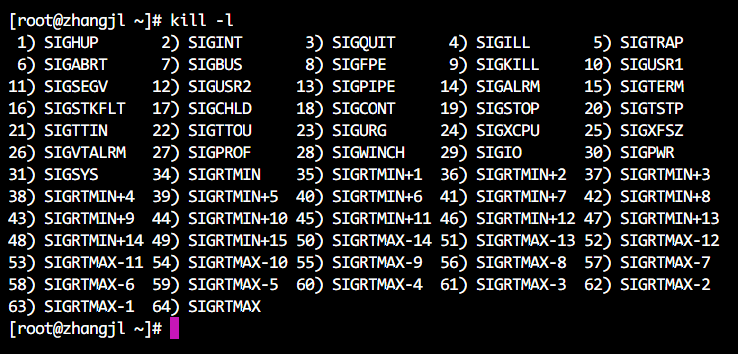
\includegraphics[scale=0.4]{signal.png}
  \caption{Linux的信号种类}
  \label{fig:signal}
\end{figure}

使用信号,可以简单的实现kill的功能。在实现kill命令功能的时候,需要使用kill函数,具体示例如下:
\begin{code-block}{c}
#include <stdio.h>
#include <stdlib.h>
#include <signal.h>

int main(int argc, char *argv[])
{
        if(argc != 3)
        {
                printf("Usage kill signal pid\n");
                return -1;
        }
        int sig = 0, pid = 0;
        sig = atoi(argv[1]);
        pid = atoi(argv[2]);
        printf("sig is %d and pid in %d\n", sig, pid);
        kill(pid, sig);
        return 0;
}
\end{code-block}

除了使用kill进行信号的发送之外,还可以使用其他的函数进行信号的发送,比如常用的的raise,alarm等;信号的接收,通常采用pause,sleep
以及while(1)等方式;而信号的处理则通常交给signal进行。

Raise函数只会发送信号给自己,基本上等价于kill(getpid(), sig),即希望通过内核给自己发信号,常用于杀掉自身的进程,如下
\begin{code-block}{c}
#include <stdio.h>
#include <signal.h>

int main(int argc, char *argv[])
{
        printf("Raise before\n");
        raise(9);
        printf("Raise after\n");
        return 0;
}
\end{code-block}

上述代码,在编译之后运行,只有before能够输出,raise调用之后,自身进程被直接杀死,因此后续的after无法输出。

而alarm函数只会发送一个定时器信号,当程序接收到定时器信号之后,会终止对应的进程,如下:
\begin{code-block}{c}
#include <stdio.h>
#include <unistd.h>

int main(int argc, char * argv[])
{
        printf("Alarm Before\n");
        alarm(9);
        while(1); //等待9秒之后,该进程自动被终止
        printf("Alarm After\n");
        return 0;
}
\end{code-block}

因此,上述代码当中,after也是无法进行输出的。

而信号的接收,处理方式则有些不同。Pause函数会直接暂停当前的进程,如下:
\begin{code-block}{c}
#include <stdio.h>
#include <unistd.h>

int main(int argc, char * argv[])
{
        printf("Pause Before\n");
        pause();
        printf("Pause After\n");
        return 0;
}
\end{code-block}

Pasue函数一旦调用,则对应的进程会直接变为暂停状态,ps -ajx可以看到状态变为S。退出暂停状态的进程,可以直接使用Ctrl+C进行,而Ctrl+C本身
发送的就是一个终止信号。

上述的信号处理,通用的方式都是终止/暂停对应的进程,很明显并不是所有的场景都需要。因此,如何进行信号处理的自定义呢?我们需要采用signal
函数。Signal函数的定义如下:
\begin{code-block}{c}
void (*signal(int sig, void (*func)(int)))(int);
\end{code-block}

其中,func为一个函数指针,指向自定义的型号处理函数。除了自定义的信号处理函数之外,func这个函数指针还可以的取值为SIG\_IGN(忽略该信号)
和SIG\_DFL(采用系统默认方式处理信号)。简单的signal函数的使用如下:
\begin{code-block}{c}
#include <stdio.h>
#include <unistd.h>
#include <signal.h>

static int quit = 0;
void handler(int signalnum)
{
        printf("Recevied signal %d\n", signalnum);
        quit = 1;
}

int main(int argc, char * argv[])
{
        signal(SIGALRM, handler);
        alarm(9);
        while(!quit);
        printf("Using self defined function to handle signal\n");
        return 0;
}
\end{code-block}

Signal函数在用于子进程的退出处理当中,是比较常用的,比如:
\begin{code-block}{c}
#include <stdio.h>
#include <unistd.h>
#include <signal.h>
#include <stdlib.h>
#include <sys/wait.h>

void handler(int signum)
{
        int i = 0;
        while( i < 5)
        {
                printf("Receved signum %d\n", signum);
                i++;
        }
}

void clean(int signum)
{
        printf("Recevied signum %d, clean up the child process\n", signum);
        wait(NULL); // 需要使用wait函数,回收对应的进程,否则,子进程会成为僵尸进程
}

int main(int argc, char * argv[])
{
        pid_t pid;
        pid = fork();
        signal(SIGUSR1, handler);
        signal(SIGCHLD, clean);
        if (0 < pid)
        {
                int i =0;
                while(1)
                {
                        printf("This is the parent process [%d]\n", i++);
                        sleep(1);
                }
        }
        if(0 == pid)
        {
                sleep(5);
                //kill(getpid(), SIGUSR1);
                raise(SIGUSR1); // 可以直接替代上面的kill函数
                exit(0); // kill(getpid(), SIGCHLD); // 在子进程当中调用exit函数
                                                     // 相当于调用了kill函数,只不过
                                                     // 发送的信号是SIGCHLD,即杀死子进程
        }
        return 0;
}
\end{code-block}

需要注意,无名管道,命名管道以及信号,都是发生在内核空间当中,并没有发生在用户空间。
除了使用上述的方式实现进程间通信之外,在Linux当中,还可以使用IPC实现。而IPC对象包含了3种方式:
\begin{itemize}
  \item 共享内存
  \item 消息队列
  \item 信号量/灯
\end{itemize}

这些IPC对象同样是在内核空间,并没有发生在用户空间,IPC类似于Linux的文件IO操作的相关思想,可以针对文件IO与IPC做一个简单的类比,
如图\nameref{fig:IPC}所示
\begin{figure}[H]
  \centering
  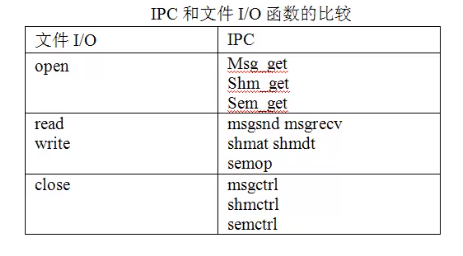
\includegraphics[scale=0.8]{IPC.png}
  \caption{文件IO与IPC的对比}
  \label{fig:IPC}
\end{figure}

\subsubsection{共享内存}
共享内存通常需要使用shmget函数进行创建,而这个函数包含3个参数:
\begin{itemize}
  \item key:IPC\_PRIVATE或者是ftok函数的返回值
  \item size:共享内存的大小,bit
  \item shmflg:共享内存的权限,同open函数
\end{itemize}
共享内存的具体使用示例如下:
\begin{code-block}{c}
#include <stdio.h>
#include <sys/shm.h>

int main(int argc, char * argv[])
{
        int shmid = 0;
        if (0 > (shmid = shmget(IPC_PRIVATE, 128, 0777)))
        {
                printf("Create shared memory failed\n");
                return -1;
        }
        return 0;
}
\end{code-block}

共享内存创建完毕之后,可以直接使用Linux提供的命令进行查看和删除。
\begin{code-block}{c}
# 查看IPC对象,包括共享内存, 或者直接ipcs
ipcs -m -q -s
# 删除IPC对象
ipcrm -m <id>
\end{code-block}
在上述代码当中,创建共享内存使用的是IPC\_PRIVATE这个宏,因此,创建出来的共享内存的
key永远为0。可以改为使用ftok函数,给不同的共享内存分配不同的标识符(key),如下:
\begin{code-block}{c}
#include <stdio.h>
#include <sys/shm.h>
#include <sys/ipc.h>

int main(int argc, char * argv[])
{
        int shmid = 0;
        int key = ftok("sharedmem.c", 's');
        if (0 > key)
        {
                printf("Failed to create shamred memory key\n");
                return -1;
        }
        if (0 > (shmid = shmget(key, 128, IPC_CREAT | 0777)))
        {
                printf("Create shared memory failed\n");
                return -1;
        }
        printf("Shared memory object id is %d\n", shmid);
        return 0;
}
\end{code-block}

IPC\_PRIVATE与ftok创建的共享内存,其关系类似与无名管道和命名管道,也就是说,IPC\_PRIVATE只能用于有亲缘关系的进程间通信,
而ftok的共享内存,则是任意进程间都可以进行通信。共享内存创建完成之后,整个是放在内核空间的,因此,用户空间无法访问,但是,
可以通过映射的方式,将共享内存将这些共享内存映射到用户空间,用户空间可以直接操作这些内存。共享内存的映射,需要使用函数shmat实现。
Shmat函数包含3个参数:id表示共享内存的id号,shmaddr表示映射的地址,NULL表示自动分配,shmflg表示映射内存的权限,0可读可写。
与管道不同,共享内存是可以反复读取的,并且,一直存在与内核当中,直到被删除或者系统关闭。

而共享内存的删除,包含了2部分的操作:1是断开与用户空间的内存映射,这个操作可以使用shmdt函数实现;2是回收内核空间当中的共享内存,
需要使用函数shmctl函数进行操作。Shmctl函数的参数如下:
\begin{itemize}
  \item hmid:表示共享内存的id
  \item cmd:表示针对共享内存的操作,可选的有3个,IPC\_STAT,获取对象属性,IPC\_SET,设置对象属性,以及IPC\_RMID删除共享内存对象
  \item buf:当cmd为IPC\_SET或IPC\_STAT时,需要使用该参数表示对象属性
\end{itemize}

共享内存的整体使用,如下示例:
\begin{code-block}{c}
#include <stdio.h>
#include <sys/shm.h>
#include <sys/ipc.h>

int main(int argc, char * argv[])
{
        int shmid = 0;
        int key = ftok("sharedmem.c", 's');
        if (0 > key)
        {
                printf("Failed to create shamred memory key\n");
                return -1;
        }
        if (0 > (shmid = shmget(key, 128, IPC_CREAT | 0777)))
        {
                printf("Create shared memory failed\n");
                return -1;
        }
        printf("Shared memory object id is %d\n", shmid);
        char * buffer = NULL;
        if (NULL == (buffer = (char *)shmat(shmid, NULL, 0)))
        {
                printf("Cannot mapping shared memory to user namespace\n");
                return -1;
        }

        fgets(buffer, 128, stdin);
        printf("Shared memory data :%s\n", buffer);

        shmdt(buffer); // 删除用户空间的共享内存映射
        buffer = NULL;

        shmctl(shmid, IPC_RMID, NULL); // 删除内核空间的共享内存

        return 0;
}
\end{code-block}

共享内存也常常用于进程间通信,比如父子进程之间的通信,如下所示:
\begin{code-block}{c}
#include <stdio.h>
#include <sys/shm.h>
#include <sys/ipc.h>
#include <unistd.h>
#include <signal.h>

void parent_handler(int signum)
{
}

void child_handler(int signum)
{
}

int main(int argc, char * argv[])
{
        int shmid = 0;
        pid_t pid = 0;
        if (0 > (shmid = shmget(IPC_PRIVATE, 128, 0777)))
        {
                printf("Create shared memory failed\n");
                return -1;
        }
        printf("Shared memory object id is %d\n", shmid);

        pid = fork();
        char * buffer = NULL;
        if (0 < pid)
        {
                signal(SIGUSR2, parent_handler);
                printf("In parent process\n");
                if (NULL == (buffer = (char *)shmat(shmid, NULL, 0)))
                {
                        printf("Cannot mapping shared memory to user namespace in parent process\n");
                        return -1;
                }
                while(1)
                {
                        fgets(buffer, 128, stdin);
                        kill(pid, SIGUSR1); // 发送信号给子进程,唤醒子进程
                        pause(); // 暂停
                }
        }

        if (0 == pid)
        {
                signal(SIGUSR1, child_handler);
                if (NULL == (buffer = (char *)shmat(shmid, NULL, SHM_RDONLY)))
                {
                        printf("Cannot mapping shared memory to user namespace in child process\n");
                        return -1;
                }
                while(1)
                {
                        pause();
                        printf("The shared memory data is %s\n", buffer);
                        kill(getppid(), SIGUSR2); //发送信号给主进程,唤醒主进程
                }
        }

        shmdt(buffer);
        buffer = NULL;

        shmctl(shmid, IPC_RMID, NULL);

        return 0;
}
\end{code-block}

共享内存也可以使用实现没有亲缘关系的进程间的通信,示例如下:
\begin{code-block}{c}
// 服务端的代码
#include <stdio.h>
#include <sys/shm.h>
#include <sys/ipc.h>
#include <signal.h>
#include <stdlib.h>
#include <unistd.h>

typedef struct _buffer{
        int pid;
        char buf[128];
}buffer_t;

void hanlder(int signum){}

int main(int argc, char * argv[])
{
        signal(SIGUSR2, hanlder);
        pid_t pid = 0;
        int shmid = 0;
        buffer_t *buffer = NULL;

        int key = ftok("server.c", 's');
        if (0 > key)
        {
                printf("Failed to create shamred memory key\n");
                return -1;
        }
        if (0 > (shmid = shmget(key, sizeof(buffer_t), IPC_CREAT | 0777)))
        {
                printf("Create shared memory failed\n");
                return -1;
        }
        if (NULL == (buffer = (buffer_t *)shmat(shmid, NULL, 0)))
        {
                printf("Mapping shared memory failed \n");
                return -1;
        }

        buffer->pid = getpid(); // 通过共享内存,向客户端发送自己的pid
        pause(); // 等待客户端的输入,等待信号SIGUSR2唤醒
        pid = buffer->pid; // 获得客户端的pid

        while(1)
        {
                printf("Server process start write share memory\n");
                fgets(buffer->buf, 128, stdin);
                kill(pid, SIGUSR1); // 使用信号SIGUSR1唤醒客户端
                pause();
        }

        shmdt(buffer);
        buffer = NULL;
        shmctl(shmid, IPC_RMID, NULL);

        return 0;
}

// 客户端代码
#include <stdio.h>
#include <sys/shm.h>
#include <sys/ipc.h>
#include <signal.h>
#include <stdlib.h>
#include <unistd.h>

typedef struct _buffer{
        int pid;
        char buf[128];
}buffer_t;

void handler(int signum){}

int main(int argc, char * argv[])
{
        signal(SIGUSR1, handler);
        int shmid = 0;
        buffer_t *buffer = NULL;

        pid_t pid = 0;
        int key = ftok("server.c", 's');
        if (0 > key)
        {
                printf("Failed to create shamred memory key\n");
                return -1;
        }
        if (0 > (shmid = shmget(key, sizeof(buffer_t), IPC_CREAT | 0777)))
        {
                printf("Create shared memory failed\n");
                return -1;
        }
        if (NULL == (buffer = (buffer_t *)shmat(shmid, NULL, 0)))
        {
                printf("Mapping shared memory failed \n");
                return -1;
        }

        pid = buffer->pid; // 通过共享内存获取服务端的pid
        buffer->pid = getpid(); // 输入客户端本身的pid
        kill(pid, SIGUSR2); // 使用信号SIGUSR2唤醒服务端

        while(1)
        {
                pause();
                printf("Client process recevied data from shared memory: %s\n",
                        buffer->buf);
                kill(pid, SIGUSR2);
        }

        shmdt(buffer);
        buffer = NULL;
        shmctl(shmid, IPC_RMID, NULL);

        return 0;
}
\end{code-block}
